
\chapter{Салат или не салат?}



Есть мнение, что Гай Юлий "Салат" Цезарь не имеет к этому самому салату с курицей никакого отношения. И этим принято бравировать, оттопыривая мизинчик. Мол, "называя Цезаря салатом, вы совершаете фактологическую ошибку, господа...". Конечно же, это полная чушь.


Сам салат изобрел повар Цезарь Кардини в США чуть меньше века назад, с чем связана забавная байка. Но суть в том, что имя "Цезарь", оно от того самого Гая Юлия. Изначально это когномен, то есть погремуха, переводящаяся как Пышноволосый или Рассекающий. И хоть наш Юлий Цезарь не был первым (Цезарями были и отец и дед как минимум), но точно самым популярным. Томушта по итогам своей жизни Салат стал богом, а его когномен Октавиан взял себе и превратил в титул правителя государства. Дальше с погонялом Цезарь гоняла большая часть императоров, а потом он мутировал в Кесарь, Царь, Кайзер и прочие знакомые нам слова, став, де-факто, синонимом правителя и во всей постантичке. И уже отсюда можно выводить личные имена, вроде "Чезаре", "Сезар", или, собственно, "Цезарь".


То есть наш придумавший салат повар, назвавший его в честь себя, сам назван в честь Гая Юлия. А значит, мы просто получаем лишнее звено в цепи, не мешающее нам выводить прямую линию приемственности между республиканским диктатором и салатом с курицей. Поэтому называйте Юлия Салатом и не парьтесь, а всех умников шлите лесом. Dixi.

\begin{figure}[h!tb] 
	\centering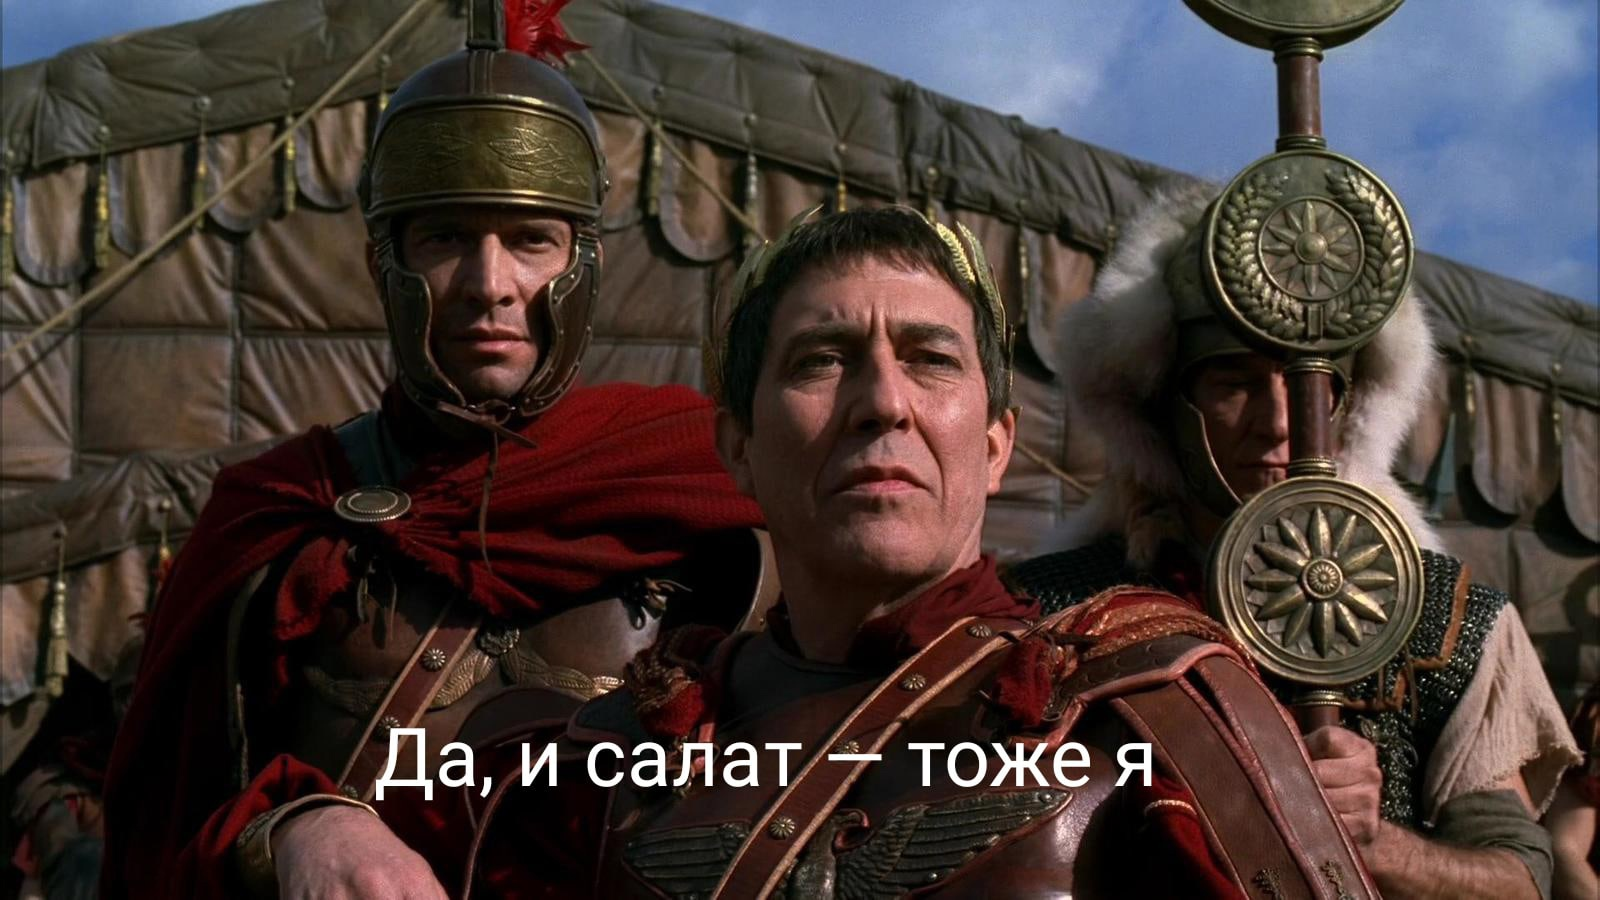
\includegraphics[scale=0.3]{Salat/161656392412378045.png}
	%	\label{fig:scipion} % Unique label used for referencing the figure in-text\end{document}
	%	%\addcontentsline{toc}{figure}{Figure \ref{fig:placeholder}} % Uncomment to add the figure to the table of contents%----------------------------------------------------------------------------------------
	%	\caption{На пикчах ниже всякие вариации на тему "сенаторы убивают Салата".}%	CHAPTER 2
\end{figure}
